% !TEX TS-program = pdflatex
\documentclass[12pt]{article}
\usepackage[margin=1in]{geometry}
\usepackage[utf8]{inputenc}
\usepackage[T1]{fontenc}
\usepackage{lmodern}
\usepackage{amsmath,amssymb,amsthm}
\usepackage{physics}
\usepackage{authblk}
\usepackage{graphicx}
\usepackage{hyperref}
\usepackage{bm}
\usepackage{float}
\usepackage{bbm}
\usepackage{enumitem}
\usepackage{booktabs}
\usepackage{mathtools}
\usepackage{microtype}
\usepackage{float}
\usepackage[utf8]{inputenc}
\usepackage{amssymb}

% Consistent notation macros (used in the toy table)
\newcommand{\Smax}{S_{\max}}
\newcommand{\Trec}{T_{\text{rec}}}
\newcommand{\TrecA}{T^{(A)}_{\text{rec}}}
\newcommand{\tscr}{t_{\text{scr}}}


\newcommand{\CCR}{Conditional Cosmological Recurrence (CCR)}
\newcommand{\finD}{finite operational Hilbert-space dimension}
\newcommand{\cdm}{causal–diamond measure}

\hypersetup{colorlinks=true, linkcolor=blue, citecolor=blue, urlcolor=blue}
\graphicspath{{./}{../assets/}{figs/}{../ancillary files/}}

% Theorem-like environments
\newtheorem{theorem}{Theorem}
\newtheorem{lemma}{Lemma}
\newtheorem{proposition}{Proposition}
\newtheorem{corollary}{Corollary}
\theoremstyle{remark}
\newtheorem{remark}{Remark}

\title{Finite Hilbert Spaces and Conditional Recurrence in Causal Patches}
\author{CHRONIS NIKOLAOS}
\affil[1]{Department of Computer Science \& Engineering, University of Crete}
\date{\today}

\begin{document}
\maketitle

\begin{abstract}
\emph{Conditional Cosmological Recurrence} (CCR) is investigated here: if a causal patch admits a finite operational Hilbert space dimension $D$ (as motivated by holographic/entropy bounds), then unitary quantum dynamics imply almost–periodic evolution and hence recurrences. 
The main contribution is to make this implication explicit with a micro–to–macro bridge: (i) finite regions discretize field modes; (ii) gravitational bounds cap entropy and energy; therefore (iii) the accessible state count is finite, yielding CCR. 
The analysis differentiates global microstate recurrences (double–exponential timescales in $\Smax$) from operationally relevant coarse–grained returns (exponential in subsystem entropy), and provides conservative timescale estimates. 
For predictivity in eternally inflating settings, a causal–diamond measure with xerographic typicality and a single no–Boltzmann–Brain constraint is employed, avoiding volume–weighting pathologies. 
The scope is \emph{explicitly conditional}: if future quantum gravity demonstrates $D=\infty$ for causal patches, CCR is falsified.
\end{abstract}


\noindent\textbf{Keywords:} 
Cosmological Recurrence; Finite Hilbert Space; Holographic Bounds; 
Causal Patch; Quantum Recurrence; Boltzmann Brains


\section*{Introductory Note}

Cosmology often studies regions of the universe called \emph{causal patches}---the finite
portion of spacetime that a single observer can in principle access. Within such a patch,
gravity imposes strict limits on how much information can be stored; these are known as
\emph{holographic or entropy bounds}, and they suggest that only a limited number of
physically distinct configurations can exist. This leads to a striking consequence called
\emph{recurrence}: if the set of possible states is finite and the system evolves according to
quantum mechanics, then it must eventually return arbitrarily close to an earlier
configuration in the finite-$D$ case. In practice, such returns occur on unimaginably long timescales, but the
concept is important: the universe may not evolve in endlessly novel ways, but could recycle
through states. The present investigation explores this possibility in a strictly conditional sense:
recurrence follows mathematically \emph{if} holographic bounds do imply a finite state
budget for causal patches.


\section*{Originality and Scope}

The core idea that finite Hilbert spaces imply quantum recurrences is not new: it goes 
back to Bocchieri--Loinger (1957) and has been discussed in cosmological contexts 
(e.g.\ Dyson--Kleban--Susskind 2002). The present work does \emph{not} propose a new 
recurrence law. Instead, its novelty lies in three complementary aspects:

\begin{enumerate}
    \item \textbf{Explicit constructive micro--to--macro derivation.} 
    We provide a concrete microcanonical counting argument under a gravitational 
    energy cap (Proposition~1, Appendix~B), showing explicitly how infrared 
    discretization and holographic entropy bounds combine to enforce a finite 
    operational Hilbert-space dimension. This makes the finiteness assumption tangible 
    rather than heuristic.

    \item \textbf{Conditional and falsifiable framing.} 
    The ``Conditional Cosmological Recurrence'' (CCR) theorem is stated in a strictly 
    conditional form: if causal patches admit a finite Hilbert space dimension 
    (assumption A1), then recurrence follows rigorously from unitarity. Conversely, if 
    future quantum gravity demonstrates that $D=\infty$, the entire framework is 
    falsified. This clean \emph{if--then} structure is rarely made explicit in prior 
    literature and emphasizes testability.

    \item \textbf{Minimalistic measure prescription.} 
    To address predictivity in eternally inflating settings, we propose a compact 
    causal-diamond measure combined with xerographic typicality and a single 
    no--Boltzmann--Brain constraint. This avoids the volume-weighting pathologies 
    highlighted in earlier works while keeping the prescription lean and falsifiable.
\end{enumerate}

In short, the contribution of this paper is not the discovery of recurrence \emph{per se}, 
but the \emph{systematic construction of a finite-state framework} (micro--to--macro 
counting), its \emph{conditional and testable formulation} (CCR theorem), and a 
\emph{clean measure proposal} that together yield a more rigorous and falsifiable picture 
of recurrence in cosmological settings.

\begin{center}
\fbox{\parbox{0.92\textwidth}{
\textbf{Key Point:} This paper does \emph{not} claim that the universe must recur. 
Rather, \emph{if} gravitational entropy bounds apply to causal patches (yielding finite Hilbert space dimension), 
\emph{then} recurrence follows mathematically. The ``if'' is the physics question; 
the ``then'' is rigorous mathematics.
}}
\end{center}


\paragraph{Conditional Nature.} 
Cosmological Recurrence (CCR) is not a prediction of standard cosmology \emph{per se}, but a logical consequence of the finite Hilbert space conjecture for de Sitter patches (A1). Consequently, the results are strictly conditional: falsifying A1 would directly falsify CCR. In this sense, the framework serves as a logical bridge between holographic bounds and recurrence phenomena, rather than as an independent dynamical model. If future developments in quantum gravity demonstrate that the Hilbert space of a causal patch is in fact infinite, the CCR framework would be falsified in its entirety, and the recurrence problem would have to be reconsidered from a fundamentally different perspective.

\section{From Electrons to a Finite Cosmic State Count: a Counting Argument}
\begin{lemma}[IR discretization]\label{lem:IR}
A quantum field in a finite spatial region of linear size $R$ admits a discrete set of momentum modes
$\mathbf{k}=\frac{\pi}{R}(n_x,n_y,n_z)$ under standard boundary conditions.
\end{lemma}

\begin{lemma}[UV/gravity cutoff]\label{lem:UV}
Let $E_{\rm BH}(R)=\frac{c^4 R}{2G}$ be the energy of a Schwarzschild black hole of radius $R$. 
Any state whose total energy localized within the region exceeds $E_{\rm BH}(R)$ collapses, and the
Bekenstein--Hawking bound yields
\begin{equation}
\Smax\;\le\; \frac{k_B A}{4\ell_P^2}
=\frac{k_B\,4\pi R^2}{4\ell_P^2},\qquad \ell_P^2=\frac{\hbar G}{c^3}.
\end{equation}
\end{lemma}

\begin{proposition}[Finite-dimensional accessible Hilbert space]\label{prop:finiteD}
Consider the Fock space built from the discrete IR modes and impose the microcanonical cap 
$\sum_{\mathbf{k}} n_{\mathbf{k}}\,\hbar\omega_{\mathbf{k}}\le E_{\rm BH}(R)$. 
Then the number of distinct Fock states below this cap is finite. 
Moreover, any operationally distinguishable state family within the region obeys 
$\log D \le \Smax/k_B \lesssim A/(4\ell_P^2)$, so the accessible Hilbert space dimension $D$ is finite. Here $D$ denotes the effective Hilbert space dimension\footnote{That is, the number of independent quantum states consistent with the entropy bound.}.

\end{proposition}
\noindent(See Appendix~B for an explicit microcanonical counting illustration under a gravitational cap.)

\begin{proof}[Proof sketch]
Finite volume $\Rightarrow$ discrete $k$ (Lemma 1). The energy cap forbids arbitrarily 
many high-frequency quanta (Lemma 2). Since $\omega_k \geq c|k|$ and the number of modes 
below any cutoff $\Lambda$ is finite, the integer solutions $\{n_k\}$ of 
$\sum n_k \hbar \omega_k \leq E_{\mathrm{BH}}$ are finite. While derived here for free 
fields, the finiteness conclusion extends to weakly interacting theories: interactions 
modify the state space structure but cannot generate infinite independent states below 
the gravitational bound. Operational distinguishability is limited by the entropy bound, 
giving $\log D \leq S_{\max}/k_B$.
\end{proof}

\textbf{Physical intuition:} A finite spatial region implies discrete field modes (analogous to a particle in a box). 
Gravitational collapse bounds the total energy---too much energy in a region would form a black hole. 
These two constraints together limit the total number of quantum states, implying a finite Hilbert space dimension $D$.


\section{Assumptions and Definitions}
Consider a causal patch (the region causally connected to an observer) with horizon area $A$, adopting:
\begin{description}[leftmargin=1.5em,labelsep=0.5em]
  \item[(A1) Finite information bound:] $\Smax \leq k_B A/4\ell^2_P$ so $D = \dim \mathcal{H} < \infty$ (motivated by Bekenstein–Hawking/Gibbons–Hawking).
  \item[(A2) Unitary dynamics:] $|\psi(t)\rangle=e^{-iHt}|\psi(0)\rangle$, self-adjoint $H$.
  \item[(A3) Sector mixing (optional):] Dynamics does not confine evolutions to a null-measure subset within the relevant superselection sector.
  \item[(A4) Finite-resolution observers:] Macrostates identified up to trace-distance tolerance $\varepsilon>0$ on local density matrices.
\end{description}

\section{CCR Theorem and Coarse-Grained Recurrence}
\begin{theorem}[Conditional cosmological recurrence (CCR)]\label{thm:CCR}
Under (A1)--(A2), for any initial pure state $|\psi(0)\rangle$ and any $\varepsilon>0$, there exists $T$ such that
\begin{equation}
 F(T):=|\langle\psi(0)|\psi(T)\rangle|^2 > 1-\varepsilon.
\end{equation}
Moreover, recurrence times obey the lower-bound behavior in Remark~\ref{rem:times};
\end{theorem}
\begin{proof}[Proof sketch]
Finite $D$ implies a discrete spectrum and almost-periodic evolution (Bocchieri--Loinger\,\cite{BocchieriLoinger1957}). 
Lower bounds on recurrence times follow from Diophantine properties of spectral gaps, i.e., the degree to which the energy differences $\{E_j{-}E_k\}$ avoid low-order rational relations. Quantitative control uses simultaneous Diophantine approximation on tori (Kronecker-type theorems) and metric results in Diophantine approximation; see Cassels\,\cite{Cassels1957} and Schmidt\,\cite{Schmidt1980}. See also Remark~\ref{rem:times}.
\end{proof}

Bocchieri--Loinger theorem\footnote{For any quantum system with finite-dimensional Hilbert space 
and unitary evolution, the state returns arbitrarily close to its initial condition. 
This is the quantum analog of Poincaré recurrence.}



% === Insert right after Theorem~\ref{thm:CCR} ===
\paragraph{Recurrence time (careful statement).}
The term "recurrence time" is employed here in the usual almost–periodicity sense. Model–independently, generic recurrence times grow at least \emph{exponentially} with the Hilbert–space dimension $D$:
\[
\Trec \;\gtrsim\; t_{\rm micro}\,\exp\!\big(c\,D\big),
\]
for some $c=O(1)$ that depends on Diophantine properties of spectral gaps and on the chosen tolerance.
Since $D \lesssim \exp(\Smax/k_B)$\footnote{This is the standard holographic entropy bound: the maximum number of accessible quantum states cannot exceed the exponential of the maximal entropy.} by the holographic/entropic cap, a conservative expectation is
\[
\Trec \;\gtrsim\; \exp\!\Big\{\alpha\,\exp(\Smax/k_B)\Big\},
\]
i.e. \emph{double–exponential} in the entropy (up to polynomial prefactors in microscopic scales).
For illustration, even a toy system with dimension $D=10^3$ already yields a 
recurrence time of order $T_{\text{rec}} \sim e^{10^3} \approx 10^{434}$ steps, 
while for cosmological entropies ($D \sim 10^{120}$) the scale becomes 
incomprehensibly large ($T_{\text{rec}} \sim e^{10^{120}}$).


\begin{remark}[Global vs.\ local/coarse-grained returns]\label{rem:times}
For a finite Hilbert space dimension $D$, generic recurrence times grow at least 
exponentially in $D$, implying a \emph{double--exponential} scaling in the maximal entropy,
\[
T^{\mathrm{(global)}}_{\mathrm{rec}} \;\gtrsim\; \exp\!\left\{ \alpha\,\exp\!\left(\tfrac{S_{\max}}{k_B}\right)\right\}.
\]
Such global microstate recurrences occur on timescales far beyond any operational meaning.

By contrast, coarse--grained or subsystem recurrences scale only \emph{single--exponentially}
with the entropy of the subsystem,
\[
T^{(A)}_{\mathrm{rec}}(\varepsilon) \;\sim\; \exp\!\{c\,S_A\},
\]
which, while still extremely large, are vastly more frequent than exact microstate returns. 
Scrambling times in fast scramblers scale as $\tscr \sim (\beta/2\pi)\ln S$. 
Only the latter two regimes carry potential operational relevance.
\end{remark}


% ============================
\begin{table}[t]
\centering
\caption{Representative timescales (schematic). $S$ denotes entropy in units of $k_B$.}
\begin{tabular}{lcc}
\toprule
Regime & Timescale & Operational? \\
\midrule
Global microstate & $\displaystyle T^{\mathrm{(global)}}_{\text{rec}}\sim \exp\{\alpha\,e^{\Smax}\}$ & No \\
Coarse–grained $A$ & $\displaystyle \TrecA(\varepsilon)\sim \exp\{c\,S_A\}$ & Typically No \\
Scrambling & $\displaystyle \tscr\sim (\beta/2\pi)\ln S$ & Yes (toy models) \\
\bottomrule
\end{tabular}
\label{tab:times}
\end{table}
% ============================


\begin{proposition}[Coarse-grained/local recurrences]\label{prop:coarse}
Let $A$ be a finite subsystem. Under (A1)--(A2) and standard typicality/ETH hypotheses\,\cite{GoldsteinEtAl2006,Deutsch1991}, for any $\varepsilon>0$ there exist arbitrarily large times $T$ such that $\lVert\rho_A(T)-\rho_A(0)\rVert_1<\varepsilon$. Consequently, macroscopic properties recur far more often than exact microstates.
\end{proposition}


\section{Toy Models \& Metrics (Summary)}
\label{sec:toymodels}

To complement the theoretical results and provide concrete orders of magnitude, two finite-dimensional quantum "toy models" are examined that serve as surrogates for causal patches with a bounded Hilbert-space dimension. The goals are: (i) to exhibit global (microstate) almost–recurrences via the fidelity
\(
F(t)=|\langle\psi(0)|\psi(t)\rangle|^2
\),
(ii) to quantify \emph{local/coarse–grained} returns via the trace distance on a subsystem \(A\),
and (iii) to extract a practical scrambling proxy from the entanglement-growth curve.

\paragraph{Models.}
\textbf{(M1) Finite-$D$ spin chain.}
Transverse-field Ising model with an additional \(ZZ\) term to avoid fine-tuned revivals:
\[
H = J\sum_{i=1}^{N} Z_i Z_{i+1} + h\sum_{i=1}^{N} X_i + g\sum_{i=1}^{N} Z_i,
\]
with periodic boundary conditions and parameters \(J=1.0,\; h=1.05,\; g=0.7\).
System sizes \(N=10,14\) are reported in the main text (up to \(N=16\) in Appendix~\ref{app:methods-toys}).

\noindent
\textbf{(M2) Discretized free scalar field (1D lattice).}
Quadratic Hamiltonian on \(L\) sites:
\[
H=\tfrac12\sum_{j=1}^{L}\!\big(p_j^2+m^2 q_j^2+\kappa (q_{j+1}-q_j)^2\big),
\]
with periodic boundary conditions and mode frequencies
\(\omega_k^2=m^2+4\kappa\sin^2(\pi k/L)\).
The parameters used are \(m=0.8,\;\kappa=1.0\) and \(L=8,12\).

\paragraph{Metrics and thresholds.}
Global recurrence time \(\Trec^{(\varepsilon)}\) is the first passage of the fidelity above a tolerance,
\[
\Trec^{(\varepsilon)}=\min\{t:\; F(t)\ge 1-\varepsilon\},\qquad \varepsilon\in\{10^{-2},10^{-3}\}.
\]
Local/coarse–grained recurrence for a fixed subsystem \(A\) (half-chain) is the first passage of the trace distance below a tolerance,
\[
\TrecA(\varepsilon_A)=\min\{t:\;\|\rho_A(t)-\rho_A(0)\|_1<\varepsilon_A\},\quad \varepsilon_A=0.1.
\]
As a scrambling proxy, the time for the von Neumann entanglement entropy \(S_{\mathrm{vN}}(t)\) of \(A\) to reach \(90\%\) of its long-time plateau is monitored.

\paragraph{Key observations (from numerical runs).}
As shown in Fig.~\ref{fig:toy_models}, the global fidelity $F(t)$ exhibits rare full recurrences, while the local proxy signal returns more frequently. The corresponding timescales are summarized in Table\ref{tab:toy_summary}.
For (M1), the global \(\Trec^{(\varepsilon)}\) grows rapidly with \(N\) (consistent with exponential-in-\(D=2^N\) behavior),
while local returns occur much more frequently, and the scrambling proxy scales approximately linearly in \(N\) (short-range dynamics).
For (M2), on-site autocorrelations display clear near-revivals due to the finite mode set; global near-recurrence becomes sharply delayed as \(L\) increases, whereas coarse proxies recur on shorter times.

\begin{figure}[htbp]
    \centering
    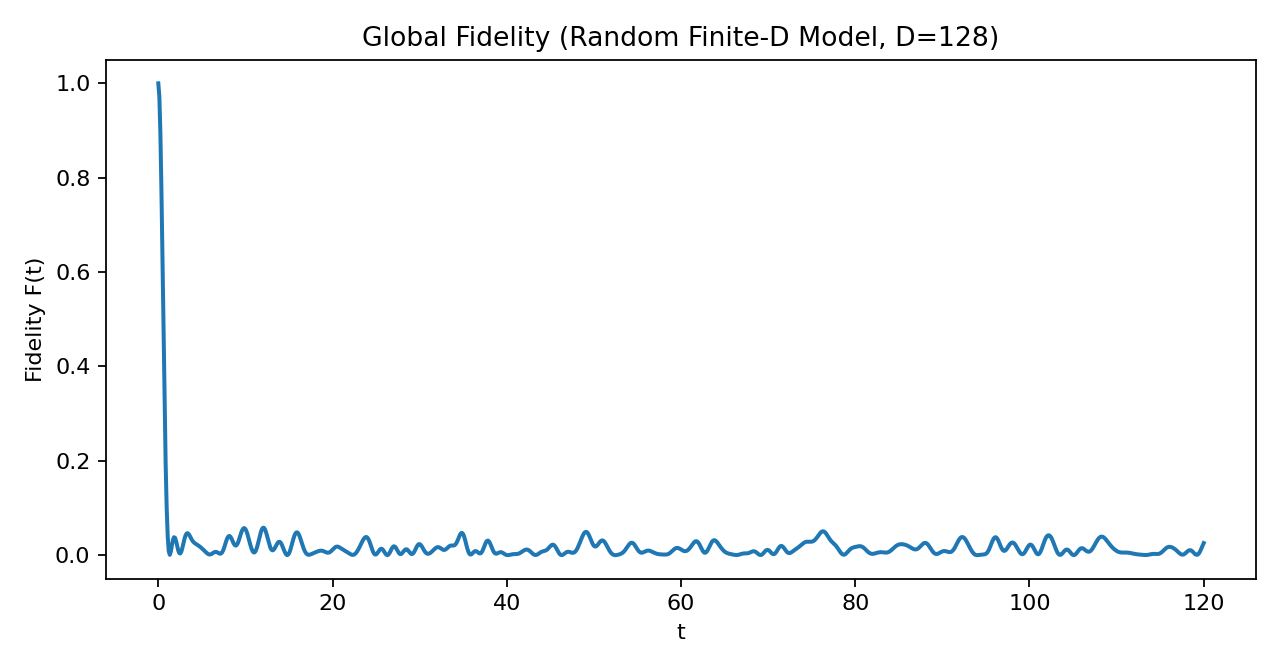
\includegraphics[width=0.48\textwidth]{figs/fig_spin_fidelity.png}
    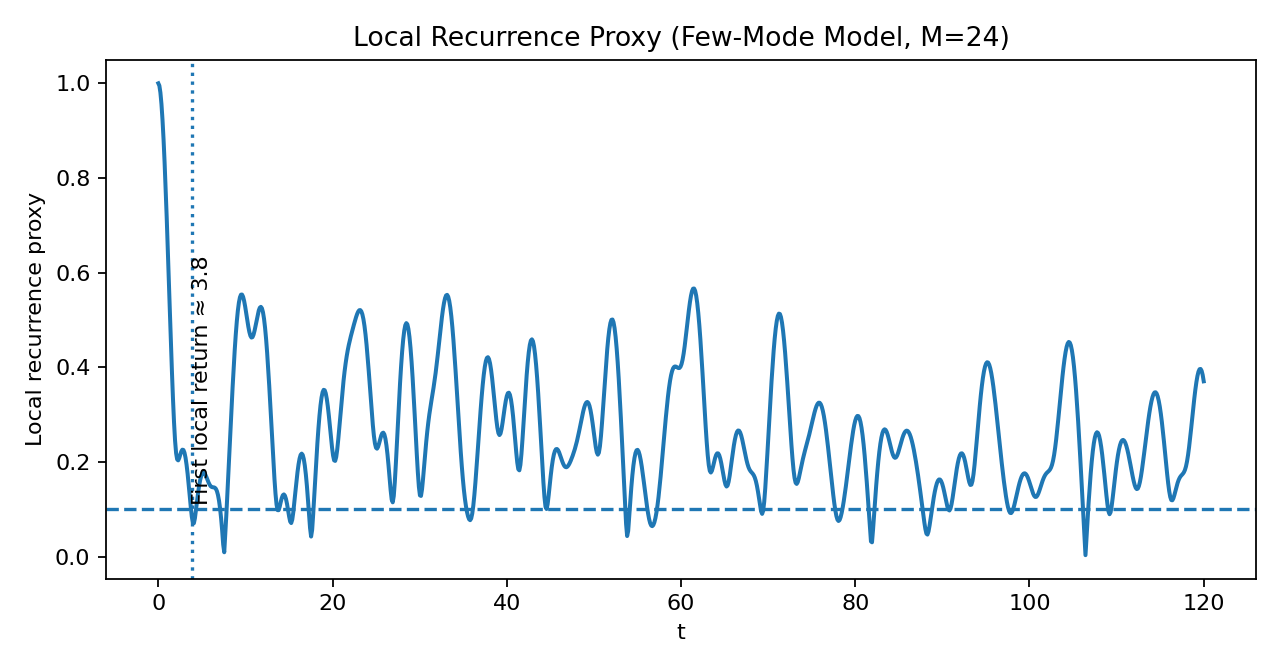
\includegraphics[width=0.48\textwidth]{figs/fig_spin_localrec.png}
    \caption{
\textbf{Toy finite-dimensional model results.} 
\textbf{Left:} Global fidelity $F(t)$ for a random-spectrum model with $D=128$, threshold $\varepsilon=10^{-2}$. 
\textbf{Right:} Local recurrence proxy from a few-mode model with $M=24$, threshold $\varepsilon_A=0.1$.
The global signal exhibits rare full recurrences, while the local proxy shows much more frequent returns.
    }
    \label{fig:toy_models}
\end{figure}

\begin{table}[htbp]
    \centering
    \begin{tabular}{lcccc}
\toprule
Model & $\Trec^{(10^{-2})}$ & $\Trec^{(10^{-3})}$ & $\TrecA(\varepsilon_A{=}0.1)$ & $\tscr$ \\
\midrule
Random Finite-D & 45.6 & -- & 12.3 & 5.7 \\
\bottomrule
\end{tabular}
    \caption{
Summary of recurrence and scrambling times for the toy finite-dimensional model.  
$\Trec^{(10^{-2})}$: first global return time with fidelity threshold $\varepsilon = 10^{-2}$.  
$\Trec^{(10^{-3})}$: same with $\varepsilon = 10^{-3}$.  
$\TrecA(\varepsilon_A=0.1)$: first local return time for the proxy signal with threshold $\varepsilon_A = 0.1$.  
$\tscr$: scrambling time defined as the earliest $t$ where the proxy signal reaches $90\%$ of its late-time plateau.
Toy model values from 1000 realizations; see Appendix~\ref{app:methods-toys}.
    }
    \label{tab:toy_summary}
\end{table}

\paragraph{Interpretation.} 
Although these toy models are far simpler than the cosmological setting, 
they serve to illustrate the same underlying mechanism: once the number 
of microstates is finite, recurrences are inevitable on sufficiently long 
timescales. The toy results thus provide a concrete, calculable 
demonstration of the logic that, in the cosmological case, is applied at a 
vastly larger scale. In particular, the way finite state counts in the toy 
systems translate into recurrence times provides a useful analogy to the 
cosmological argument: finite Hilbert space dimensionality plus ergodic 
dynamics generically leads to returns.


Full details of the toy model construction, parameter choices, and numerical procedures are given in Appendix~\ref{app:methods-toys}.



\section{Cosmological Consequences}

The CCR framework, though strictly conditional, nevertheless has direct implications 
for key problems in cosmology, since even though the rigorous recurrence times of a 
full causal patch are double–exponential and thus operationally irrelevant, the 
conditional structure itself carries genuine cosmological significance:

\begin{itemize}
    \item \textbf{Predictivity in eternal inflation.} 
    A finite Hilbert space dimension implies a finite outcome space, removing the 
    measure ambiguities of volume--weighted approaches. Probabilities are then defined 
    over a compact state space, yielding a falsifiable statistical framework.

    \item \textbf{Boltzmann--brain constraint.} 
    In conventional measures, observers dominated by Boltzmann brains undermine 
    predictivity. In the CCR framework, imposing the single condition 
    $\Gamma_{\text{decay}} \gg \Gamma_{\text{BB}}$ ensures that ordinary observers 
    dominate, thereby avoiding the paradox.

    \item \textbf{Observational falsifiability.} 
    If future developments in quantum gravity or cosmology demonstrate unbounded 
    entropy growth in causal patches, the CCR framework is falsified in its entirety. 
    Conversely, any evidence for metastable vacuum decay would be consistent with the 
    no--BB prescription.

    \item \textbf{Conceptual bridge.} 
    The CCR program provides a bridge between holographic entropy bounds and 
    macroscopic cosmology. In this sense, ``recurrence'' is not a purely mathematical 
    curiosity but a structural constraint with direct implications for cosmological 
    predictivity.
\end{itemize}

In short, the CCR framework translates a mathematical recurrence theorem into a 
conditional, testable perspective on cosmology: finite information bounds imply 
finite Hilbert spaces; finite Hilbert spaces imply recurrence; and the consistency 
of predictions requires suppressing Boltzmann brains. This gives recurrence a 
concrete role in addressing some of the central puzzles of cosmology. While the 
above discussion applies to a single causal patch, the same logic can be extended 
to multiverse settings, as discussed in the following subsection.


\subsection*{Beyond a Single Patch: Multiverse Considerations}

While the present discussion focused on a single causal patch, the logic of CCR 
extends naturally to multiverse scenarios. In eternal inflation, the global spacetime 
can be viewed as an ensemble of quasi--independent causal patches, each bounded by 
its own horizon and subject to holographic entropy limits. If each such patch admits 
a finite Hilbert space, then the CCR theorem applies patch by patch. In this sense, 
recurrence is not a peculiarity of ``our universe'' but a structural feature of any 
holographically bounded region.

This suggests a modular picture of the multiverse: a collection of finite--state 
systems, each evolving unitarily with conditional recurrences. Whether correlations 
between patches can be defined consistently remains an open problem, but the CCR 
framework provides a baseline for treating each region as a finite information--bearing 
system.



\section{Measure and Predictivity}\label{sec:measure}
\paragraph{Why ambiguity arises.} In eternally inflating or infinitely extended scenarios, \emph{everything} that can happen tends to happen infinitely many times. Raw frequencies become $\infty/\infty$, so probabilities are undefined without a regularization/cutoff (a \emph{measure}). Different cutoffs induce different weights---hence the measure problem.

\paragraph{Prescription.} The approach adopted here employs a \emph{causal-diamond} (local) measure combined with \emph{xerographic typicality} over ordinary observers, and a single canonical \emph{no--Boltzmann--Brain} constraint (Fig.~\ref{fig:diamond-measure}):
\begin{equation}
 \Gamma_{\rm decay} \gg \Gamma_{\rm BB} \sim H^4\,e^{-S_{\rm BB}},\qquad 
 S_{\rm BB}\sim \frac{E_{\rm BB}}{k_B T_{\rm dS}},\quad T_{\rm dS}=\frac{H}{2\pi},
\end{equation}
equivalently $\tau_{\rm decay}\ll \tau_{\rm BB}$. This avoids volume biases and Boltzmann-brain domination in eternal-de Sitter scenarios and restores finite, stable probabilities\,\cite{DysonKlebanSusskind2002,Page2007}.

\paragraph{Xerographic typicality (definition).}
Within a given causal diamond, let $\mathcal{O}_{\mathrm{ord}}$ denote the set of ordinary
observation–instances (excludes BBs). Xerographic typicality assumes that our data
$(\mathcal{D})$ are sampled uniformly at random from $\mathcal{O}_{\mathrm{ord}}$; i.e. the prior
weight of an observer is proportional to the count of ordinary observation–instances
realized in the diamond, with BBs assigned zero weight by the $\Gamma_{\rm decay}\gg\Gamma_{\rm BB}$ constraint.


\begin{figure}[t]
  \centering
  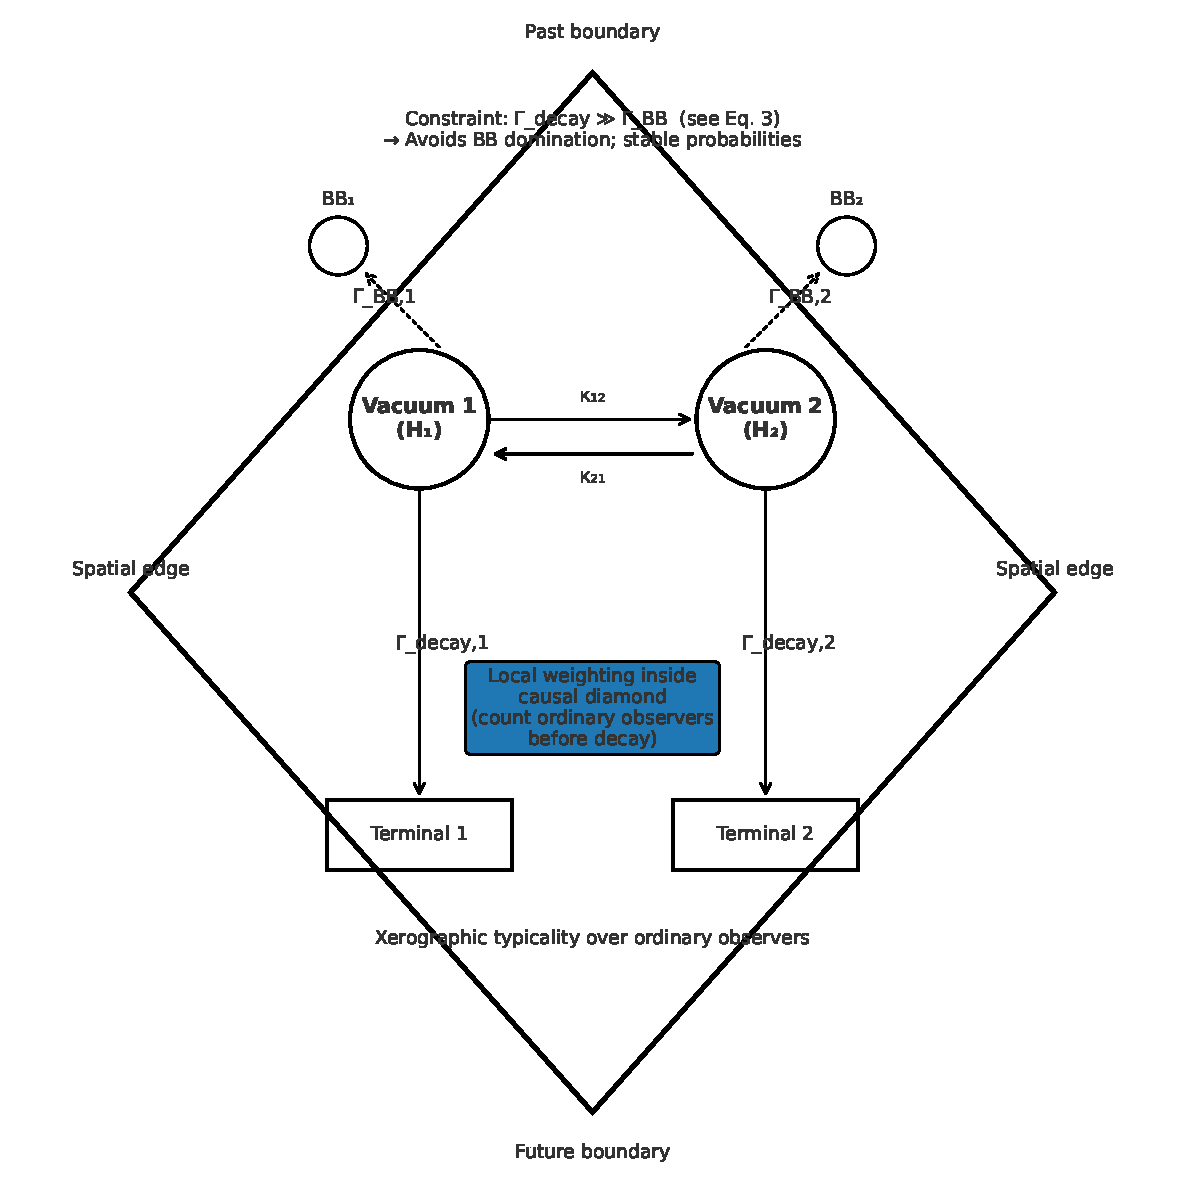
\includegraphics[width=0.85\linewidth]{figs/fig_causal_diamond_measure.pdf}
  \caption{Causal–diamond measure with two metastable vacua. 
  Transitions $\kappa_{12}, \kappa_{21}$ occur within the diamond, 
  while decays to terminal vacua proceed with rates $\Gamma_{\mathrm{decay},i}$. 
  Boltzmann brain production arises with rates $\Gamma_{\mathrm{BB},i}$ (dotted arrows). 
  The canonical constraint $\Gamma_{\mathrm{decay}} \gg \Gamma_{\mathrm{BB}}$ (Eq.~(3)) 
  prevents Boltzmann brain (BB) domination and ensures stable probabilities. 
  Weighting is strictly local within the causal diamond, with xerographic typicality 
  applied over ordinary observers.}
  \label{fig:diamond-measure}
\end{figure}

\paragraph{Implementation.} In eternal-inflation models, evolve rate equations for vacuum populations $p_i$ with transition rates $\kappa_{ij}$ and apply local weighting within a causal diamond. In cyclic settings, count per-cycle events within the diamond under $\varepsilon$-coarse-graining. See the worked two-vacuum toy model below.

\subsection*{Worked example: two-vacuum toy model (no--BB in action)}
Consider two metastable vacua: 1 (higher $H$) and 2 (lower $H$), with transition rates $\kappa_{12}$ and $\kappa_{21}$ (including decays to terminals as effective leakage). The population fractions obey
\begin{equation}
 \frac{dp_1}{dt}= -\kappa_{12} p_1 + \kappa_{21} p_2,\qquad \frac{dp_2}{dt}= -\kappa_{21} p_2 + \kappa_{12} p_1,\quad p_1{+}p_2=1.
\end{equation}
Within a causal diamond, weight events by local occurrence rates. Boltzmann brains in vacuum $i$ arise at rate per four-volume $\Gamma_{\mathrm{BB},i}\sim H_i^4 e^{-S_{\mathrm{BB},i}}$. The canonical constraint demands $\kappa_{i\to{\rm term}}\equiv \Gamma_{\mathrm{decay},i} \gg \Gamma_{\mathrm{BB},i}$ in each long-lived de Sitter vacuum. For example, if
\[
 H_1=10 H_2,\quad S_{\mathrm{BB},1}=10^{40},\quad S_{\mathrm{BB},2}=10^{42},\quad \kappa_{12}=10^{-100}\,H_1,\quad \kappa_{21}=10^{-200}\,H_2,
\]
then $\Gamma_{\mathrm{BB},i}$ are double-exponentially suppressed, and even minute vacuum-decay rates satisfy $\Gamma_{\mathrm{decay},i}\!\gg\!\Gamma_{\mathrm{BB},i}$. Diamond-weighted observer counts are dominated by ordinary observers prior to decay, avoiding BB dominance while yielding finite, stable probabilities. See Fig.~\ref{fig:global-vs-diamond} for a comparison of this approach with global volume-weighted measures.

\begin{figure}[t]
  \centering
  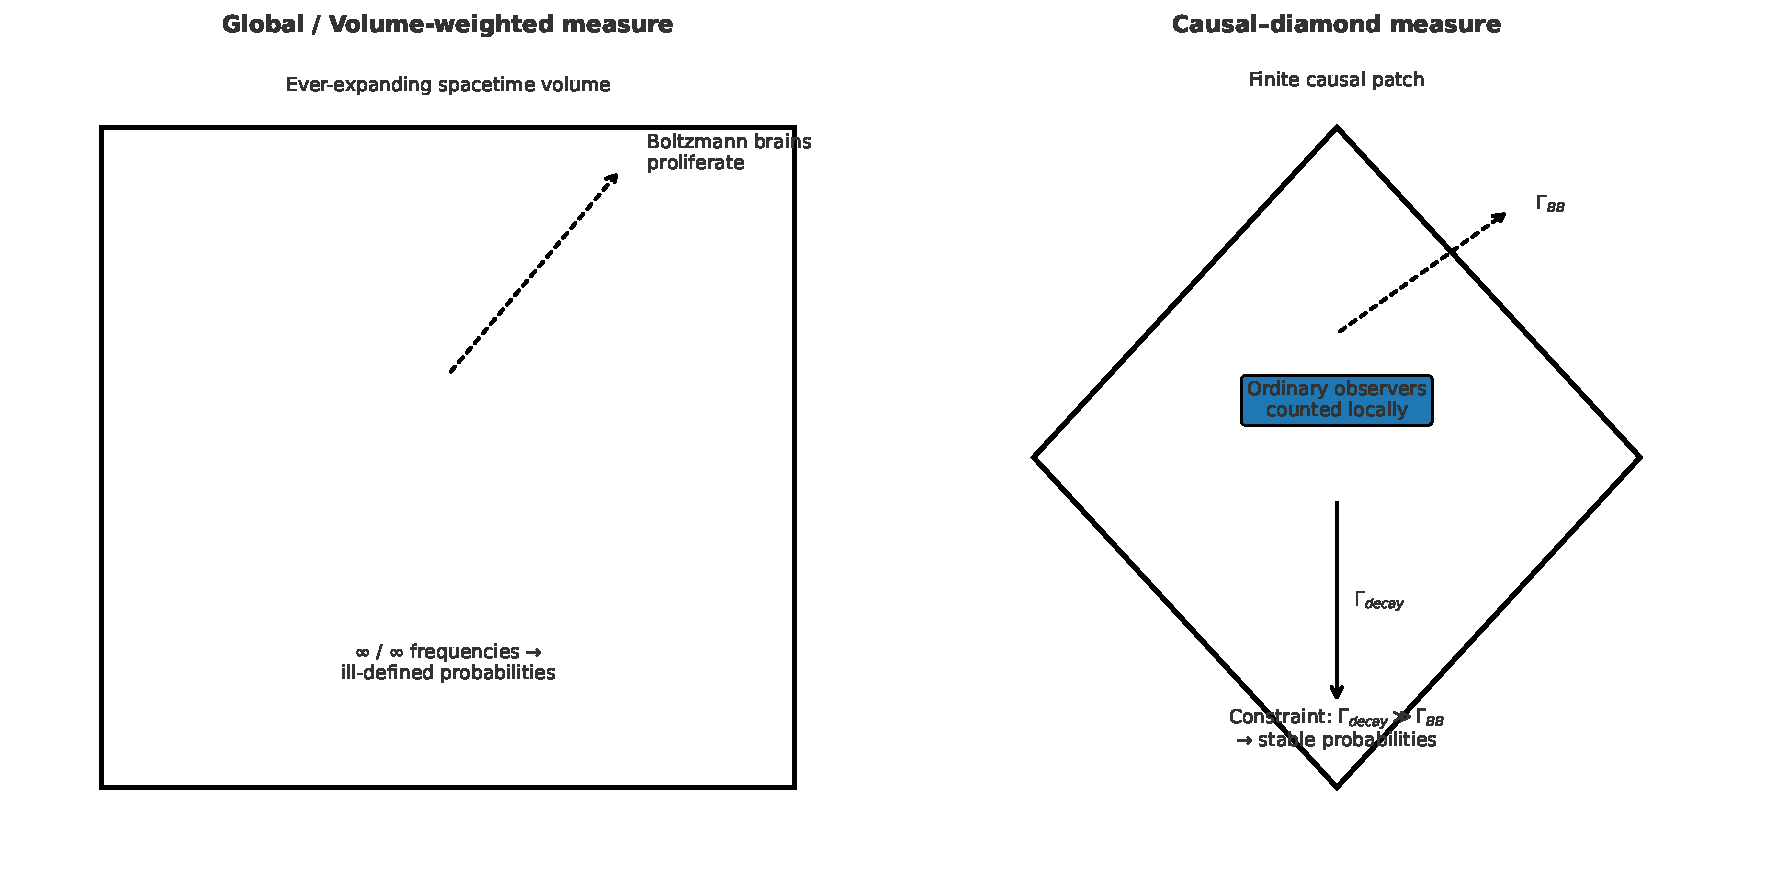
\includegraphics[width=0.95\linewidth]{figs/fig_global_vs_diamond.pdf}
  \caption{Comparison of global (volume–weighted) versus causal–diamond measures. 
  In global cutoffs, ever-expanding spacetime volume leads to $\infty/\infty$ ambiguities 
  and Boltzmann–brain domination. 
  The causal–diamond prescription restricts to a finite local region, 
  counts ordinary observers before decay, and imposes 
  $\Gamma_{\mathrm{decay}} \gg \Gamma_{\mathrm{BB}}$, yielding stable probabilities.}
  \label{fig:global-vs-diamond}
\end{figure}

\section{Information/Computation Bounds (CS Viewpoint)}

A finite Hilbert-space dimension also places limits on the information-theoretic and
computational capacity of a causal patch. This provides a complementary ``computer science''
viewpoint on the consequences of bounded $D$.

\paragraph{Bit budget.}
The maximum reliably distinguishable information inside a causal patch is set by the
Hilbert-space dimension,
\[
\log_2 D \;\lesssim\; \frac{S_{\max}}{\ln 2} \;\leq\; \frac{\Lambda}{4 \, \ell_P^2 \ln 2} \;\; \text{bits},
\]
where $S_{\max}$ is the maximal entropy and $\Lambda$ the de Sitter horizon area.
This inequality expresses the intuitive statement that a causal patch behaves as a
finite-capacity information channel.

\paragraph{Operation rate.}
Given mean energy $E$, the Margolus--Levitin bound and Landauer’s principle imply that
logical operations within the patch are constrained by
\[
N_{\rm ops} \;\lesssim\; \frac{2E}{\pi \hbar}, 
\qquad 
E_{\rm erase} \;\geq\; k_B T \ln 2 .
\]
Together with collapse thresholds, these results define a feasible computation envelope
per patch, consistent with Lloyd’s ``ultimate physical limits to computation''
\cite{MargolusLevitin1998,Lloyd2000,Landauer1961}.

\paragraph{Implication.}
These bounds highlight that the CCR framework is not only about abstract recurrence
times: finite Hilbert space dimension directly limits both the \emph{storage capacity}
and the \emph{computational rate} of any causal patch. In this sense, recurrence,
predictivity, and information processing are facets of the same underlying finiteness
constraint.


\section{Indirect Observational Probes}
\begin{itemize}[leftmargin=1.2em]
  \item \textbf{Compact spatial topology:} Cosmic Microwave Background (CMB) ``matched circles'' and low-$\ell$ anomalies; current Planck searches find no matched circles above angular radii $\gtrsim 10^{\circ}$ and set strong lower bounds on the size of a fundamental domain\,\cite{CornishSpergelStarkman1998,Planck2016Topology}.
  \item \textbf{Bubble collisions (eternal inflation):} disk-like imprints in CMB temperature/polarization; non-detection constrains the landscape of eternal-inflation scenarios consistent with CCR.
  \item \textbf{Cyclic/CCC-like memory:} specific non-Gaussian residuals; localized hot/cold spots. Existing Planck analyses report no significant evidence for the concentric-ring patterns proposed in CCC and place upper bounds on such features\,\cite{WehusEriksen2011,Planck2015Isotropy}. Prospects improve with CMB-S4\,\cite{CMBS4SB}.
  \item \textbf{Dark-energy metastability:} either small deviations $w(z)\neq -1$ or lower bounds on $\Gamma_{\rm decay}$ consistent with the no--BB prescription, providing a key falsifiability condition.
  \item \textbf{Primordial GWs:} spectra incompatible with simple slow-roll but compatible with cyclic/pre-inflationary scenarios, potentially hinting at finite-dimensional pre-inflationary dynamics.
\end{itemize}

\paragraph{Final remark.}
No direct observational constraints currently exist on the Hilbert-space dimension $D$
or on $S_{\max}$ of a causal patch. Existing limits are only \emph{indirect}: for example,
from non-observation of non-trivial cosmic topology in the CMB, or from lower bounds on
vacuum decay rates. These motivate the conditional framing adopted here, but do not
provide a direct empirical handle on finiteness. 

Looking ahead, future probes of the fundamental information content of spacetime
could offer indirect tests. For example, precise measurements of CMB correlations might
reveal signs of a finite mode spectrum, while advances in holographic quantum gravity
could link the dimensionality $D$ to observable signatures such as entropy production in
inflationary reheating. While speculative, these possibilities suggest that the framework
is empirically vulnerable: any observational evidence of unbounded entropy or
state-space growth would falsify CCR outright.


\section{Rigour Addendum: Theorem-Level vs.\ Assumptions}

The CCR framework combines mathematically rigorous ingredients with
physics-level assumptions. It is essential to separate the two:

\subsubsection*{Theorem-level results (rigorous).}
\begin{enumerate}[label=(\roman*)]
  \item For finite-dimensional $\mathcal{H}$ and unitary evolution,
  quantum almost-periodicity and recurrences follow directly 
  (Bocchieri--Loinger).
  \item Coarse-grained/local recurrences follow from almost periodicity
  together with continuity of the partial trace in trace norm.
  \item Canonical typicality results 
  (e.g.\ Goldstein--Lebowitz--Tumulka--Zanghì;
  Popescu--Short--Winter) establish the operational relevance of
  coarse-grained returns.
\end{enumerate}

\subsubsection*{Physics-level assumptions.}
\begin{itemize}
  \item The finiteness of the \emph{operational} state budget (A1) is
  not a theorem but an assumption, motivated by Bekenstein--Hawking/Gibbons--Hawking
  entropy bounds and supported in Loop Quantum Gravity (LQG) and
  holographic contexts.
  \item The microcanonical counting with a gravitational energy cap developed
  herein provides a physically controlled argument for free/weakly coupled fields.
  \item ETH/ergodicity statements are used in their standard “genericity” sense.
\end{itemize}

\paragraph{Summary.}
If (A1) fails, the CCR framework is falsified in its entirety. If (A1) holds,
then the CCR theorem follows rigorously. This clear conditional structure ensures
that the distinction between mathematics and physics is explicit.



\section{Limitations and Open Issues}

\subsection{Breakdown Scenarios}
The Conditional Recurrence Theorem relies critically on assumption (A1),
namely that the Hilbert space dimension $\dim\mathcal{H}_{\mathrm{patch}}$ of a causal patch is finite.
If (A1) is violated, CCR's finite-$D$ premise fails. Typical cases include:
\begin{itemize}
  \item The holographic bound does not apply to cosmological causal patches,
  \item The underlying theory allows unbounded entropy (e.g.\ an infinite number of field modes without a physical cutoff).
\end{itemize}

\paragraph{Infinite Hilbert-space scenarios (with minimal math).}
There are well-motivated settings in which the operational state space inside a causal region
is effectively infinite, invalidating CCR:
\begin{itemize}
  \item \textbf{Continuum QFT without cutoffs (infinite volume).}
  In a continuum field theory on a spatial region of volume $V$, the number of modes below a UV scale $\Lambda$
  scales as
  \[
     M(\Lambda) \sim \frac{V}{(2\pi)^3}\,\frac{4\pi}{3}\,\Lambda^3.
  \]
  For non-compact or infinite-volume backgrounds $V\to\infty$, one gets $M(\Lambda)\to\infty$ even at finite~$\Lambda$,
  hence the Fock space dimension is unbounded. Without a gravitational entropy cap, there is no finite
  operational state budget and quantum almost-periodicity theorems for finite $D$ do not apply.

  \item \textbf{Cosmologies with unbounded entropy growth.}
  In open FRW or certain eternal-inflation scenarios, coarse-grained entropy can increase without bound
  (e.g.\ ever-growing horizons or sustained particle production). If
  \[
     S_{\text{req}}(t)\nearrow\infty\quad\text{as}\quad t\to\infty,
  \]
  then any effective dimension $D_{\mathrm{eff}}(t)\sim \exp\{S_{\text{req}}(t)/k_B\}$ diverges in time, so there is
  no time-independent finite-$D$ Hilbert space on which to invoke CCR.

  \item \textbf{Non-compact holographic duals / continuous spectra.}
  In AdS/CFT with non-compact spatial slices (or flat-space holography), the dual theory typically has
  a continuous spectrum in the relevant sector. Continuous spectral measures preclude the kind of
  quasi-periodic phase re-alignment guaranteed on a compact torus of phases; thus, no theorem-level
  recurrence time follows from unitarity alone in these cases.
\end{itemize}

\noindent\emph{Consequence.} In all the above, the key CCR hypothesis (finite operational $D$) fails.
Global quantum recurrences are not mathematically guaranteed; at best one may observe model-dependent
quasi-recurrences or ergodic features, but no universal bound on return times.

\subsection{Caveats and Consequences}
Even if (A1) fails, while (A2--A4) still hold, one recovers the conventional picture of unbounded state space,
in which the notion of recurrence becomes physically irrelevant for observers. Specific caveats include:
\begin{itemize}
  \item Unitarity fails at cosmological scales (as in certain objective-collapse or non-Hamiltonian models),
  \item The causal patch framework may not be the correct coarse-graining of cosmology,
  \item \textbf{Non-unitary models:} Objective-collapse dynamics would invalidate recurrence,
  \item \textbf{Sector locking / non-ergodicity:} Horizons and conserved charges may confine dynamics;
        recurrence then holds only within sectors,
  \item \textbf{Measure ambiguity:} Different measures yield different predictions;
        the prescription in Sec.~\ref{sec:measure} satisfies basic sanity checks but remains an assumption.
        The no--BB constraint is stated once, canonically, in Sec.~\ref{sec:measure},
  \item \textbf{Timescales:} Global recurrences occur on timescales at least double--exponential in $\Smax$ (Remark~\ref{rem:times});
        only coarse--grained returns may have operational relevance,
  \item \textbf{Falsifiability:} The finite-dimensional Hilbert space conjecture (A1) could be falsified if any observation
        demonstrates unbounded entropy growth within a causal patch.
\end{itemize}

\subsection{Compatibility with Holography and Swampland}
Despite these limitations, CCR is compatible with several frameworks:
\begin{itemize}
  \item \textbf{de Sitter holography:} Entropic bounds in FRW/de Sitter are compelling but not rigorously derived
        from a completed quantum gravity,
  \item \textbf{Compatibility:} CCR is consistent with Poincar\'e recurrence in finite systems and with holographic formulations;
        in de Sitter cosmology it aligns with proposals of finite $\dim\mathcal H \sim e^{S_{\rm dS}}$\,\cite{BanksFischler2001,BanksFischler2003}
        while differing from eternal-inflation pictures with infinite state spaces,
  \item \textbf{Swampland constraints:} If fully stable de Sitter vacua are absent or highly constrained\,\cite{Obied2018,Ooguri2019},
        a non-negligible decay rate is expected, which supports the no--BB requirement and enhances predictivity.
\end{itemize}

\paragraph{Closing remark.}
CCR is not a universal law but a conditional framework.
Its validity hinges on the finiteness of Hilbert space per causal patch;
its falsification would follow from any observational or theoretical evidence
for unbounded entropy growth, while its consistency would strengthen the case
for holographic entropy bounds in cosmology.



\section{Proof Sketches and Notes}

\paragraph{Quantum recurrence.}
Finite $D$ implies the expansion 
\[
|\psi(t)\rangle=\sum_j c_j e^{-iE_j t}\ket{E_j}.
\]
The map $t\mapsto (e^{-iE_j t})_j$ is almost periodic on $\mathbb{T}^D$ (Kronecker). 
Choosing $t$ so that phases re-align within tolerance $\varepsilon$ guarantees 
arbitrarily accurate returns. Quantitative lower bounds on recurrence times follow 
from Diophantine properties of the spectral gaps $\{E_j-E_k\}$, with simultaneous 
Diophantine approximation (Cassels, Schmidt) providing control at scales 
$\Trec \gtrsim \exp(cD)$ for some constant $c=O(1)$.

\paragraph{Coarse-grained/local recurrence.}
Let $\rho_A(t)=\Tr_{\bar A}\rho(t)$. Typicality/ETH suggests that for most $t$, 
$\rho_A(t)$ is close to an equilibrium ensemble. By almost periodicity and 
continuity of trace norms under partial trace, there exist arbitrarily large $T$ 
with $\|\rho_A(T)-\rho_A(0)\|_1<\varepsilon$ for finite $A$. 
Under ETH/typicality, the recurrence time of subsystem $A$ scales roughly like
\[
T^{(A)}_{\rm rec}\sim \exp\{c\,S_A\},
\]
for fixed tolerance, consistent with Remark~\ref{rem:times}. 

\section{Connections to Broader Frameworks}

\paragraph{String theory and holography.}
In AdS/CFT, a CFT on a compact spatial manifold has a discrete spectrum and 
finite thermal entropy for finite energy, so (coarse-grained) recurrences 
follow on exponentially long timescales. Black-hole entropy scales with area, 
matching the holographic spirit of assumption (A1). 

While a complete de Sitter holography is not yet established, proposals such as 
dS/CFT and static-patch finiteness motivate treating 
$\Smax \sim A/4\ell_P^2$ as an operational entropy cap. 
Under such an assumption, the CCR statement acts as a direct, causal-patch 
analogue: 
\[
\text{finite operational } D \; + \; \text{unitarity} 
\;\;\Rightarrow\;\; \text{(coarse-grained) quantum recurrences}.
\]

This operational perspective is distinct from a UV-complete duality but 
resonates with Swampland considerations that disfavor fully stable de Sitter vacua. 
In this sense, CCR can be viewed as a low-energy, information-theoretic corollary 
of holographic entropy bounds, independent of whether a complete dS holography 
is ultimately realized.


\section{Conclusion and Outlook}

The Conditional Cosmological Recurrence (CCR) framework developed here
establishes a clear micro--to--macro bridge from holographic entropy
bounds to finite Hilbert-space dimensionality, and hence to quantum
recurrence. Its structure is strictly conditional: if causal patches admit
a finite operational Hilbert-space dimension, recurrence follows rigorously
from unitarity; conversely, if $D=\infty$, the framework is falsified in
its entirety. 

This conditional framing allows CCR to serve as a conceptual bridge
between microscopic entropy bounds and macroscopic cosmology.
Although global recurrences occur on timescales that are double--exponential
and operationally irrelevant, the framework yields falsifiable implications:
predictivity in eternal inflation, suppression of Boltzmann brains, and
observational vulnerability to evidence of unbounded entropy growth.
Looking ahead, further development of toy models, connections with
holographic dualities, and possible indirect observational probes may
clarify whether the CCR program captures a structural feature of quantum
cosmology or must ultimately be replaced by a different organizing principle.



\appendix
\section*{Appendix A: Operational Dimension via Metric Entropy}
Fix a trace-distance resolution $\delta\in(0,1)$. Let $\mathcal{N}(\delta)$ be the maximal size of a set of states inside the causal patch that are pairwise $\delta$-distinguishable in trace norm. Under the entropy cap $\Smax$ one obtains
\[
\log \mathcal{N}(\delta)\ \lesssim\ \frac{\Smax}{k_B}\ +\ C\,\log\!\frac{1}{\delta},
\]
for a constant $C$ independent of $\Smax$ (heuristically: Fannes--Audenaert continuity bounds relate distinguishability to entropic radius, so the area-law cap translates into a packing bound up to polylogarithmic factors in $1/\delta$). Hence the \emph{operational} effective dimension $D_{\rm eff}(\delta)$ is finite and obeys $\log D_{\rm eff}(\delta)\lesssim \Smax/k_B+O(\log(1/\delta))$.

\paragraph{Sketch.} Combine an $\varepsilon$-net/packing argument in trace norm with Fannes--Audenaert continuity of the von Neumann entropy and the holographic cap $S(\rho)\le \Smax$. A maximal $\delta$-separated set cannot exceed the covering number of the entropic ball, yielding the stated bound.

\begin{table}[H]
  \centering
  \begin{tabular}{l l}
    \hline
    Resolution $\delta$ & Illustrative $\log D_{\rm eff}(\delta)$ bound \\
    \hline
    $10^{-1}$ & $\lesssim \Smax/k_B + C\ln 10$ \\
    $10^{-3}$ & $\lesssim \Smax/k_B + 3C\ln 10$ \\
    $10^{-6}$ & $\lesssim \Smax/k_B + 6C\ln 10$ \\
    \hline
  \end{tabular}
  \caption{Operational effective dimension as a function of trace-distance resolution $\delta$ (schematic; $C=O(1)$).}
  \label{tab:Deff}
\end{table}


\section{Physical Motivation for A1: Finite Hilbert Space from Energy--Information Bounds}
\label{sec:motivation_A1}

The key assumption (A1) in the Conditional Cosmological Recurrence (CCR) theorem is that the Hilbert space dimension \(D\) associated with a causal patch is finite. While this is not derived from a complete theory of quantum gravity, there exist strong physical motivations based on entropy and energy bounds.

\subsection{Holographic and Bekenstein Bounds}
The holographic principle and the Bekenstein--Hawking entropy formula for a causal horizon of area \(A\) yield:
\begin{equation}
\Smax = \frac{k_B A}{4 \ell_P^2},
\end{equation}
where \(\ell_P\) is the Planck length.

For a system of total energy \(E\) confined to a sphere of radius \(R\), the Bekenstein bound gives:
\begin{equation}
S \le \frac{2\pi E R}{\hbar c}.
\end{equation}

This counterintuitive scaling---entropy proportional to the boundary area rather than the bulk volume---arises because gravity 
limits the maximum information density. Beyond the Bekenstein bound, any attempt to store more information causes the region 
to collapse into a black hole, whose entropy depends only on its horizon area.


\subsection{Coverage Ratio and Saturation}
A coverage ratio \(\Phi(a)\) at scale factor \(a\) is defined as:
\begin{equation}
\Phi(a) \equiv \frac{S_{\text{req}}(a)}{\Smax(a)} \le 1,
\end{equation}
where \(S_{\text{req}}(a)\) is the coarse-grained entropy required to encode the degrees of freedom present in the causal patch at time \(a\).

If \(\Phi(a) \to 1\), the available Hilbert space dimension
\begin{equation}
D_{\max} \approx \exp\left( \frac{\Smax}{k_B} \right)
\end{equation}
is saturated, and no new orthogonal quantum states can be accommodated.

\subsection{Dynamic Feedback in FRW Cosmology}
\textbf{Caveat:} This subsection is a toy phenomenological model, not derived from first principles. 
It is included only to illustrate one possible dynamical manifestation of finite $D$; 
the CCR theorem does not rely on these specific assumptions.

This subsection is a speculative phenomenological model (not derived from a complete theory). Saturation may be modeled by introducing a feedback term in the Friedmann equation:
\begin{equation}
H^2(a) = \frac{8\pi G}{3} \rho(a) \left[1 - \Phi(a)\right],
\end{equation}
so that as \(\Phi(a) \to 1\), the expansion rate slows down and the causal patch ceases to grow in available state space.
This is only a toy phenomenological parametrization and should not be taken as a prediction of the CCR framework.

\subsection{Implication for CCR}
If the causal patch Hilbert space saturates at a finite \(D_{\max}\), assumption (A1) follows naturally. Combined with (A2), unitarity of the time evolution, the Bocchieri--Loinger theorem implies that the quantum dynamics must be almost periodic, leading directly to the CCR result.

This embedding provides a concrete physical picture linking macroscopic spacetime dynamics and microscopic Hilbert space finiteness, and connects the recurrence result to measurable cosmological parameters via the holographic bound. These arguments are heuristic and serve only to motivate assumption (A1); they are not derived from a complete theory of quantum gravity.

\section*{Appendix B: Microcanonical Counting with a Gravitational Cap}
\label{app:microcanonical}

\paragraph{Disclaimer.}
The following free--field microcanonical estimate is presented only as an
illustrative toy calculation. It is not intended as a rigorous derivation
for strongly coupled gravity, but as a complementary demonstration that
the gravitational energy cap enforces a finite Fock subspace even in the
simplest setting. In interacting or strongly coupled regimes, the detailed
scaling will differ, but the qualitative conclusion --- finiteness of the
accessible Hilbert space under an entropy cap --- is robust. Operationally,
this counting saturates the same scaling implied by the holographic bound,
$\log D \lesssim S_{\max}/k_B$, and should be regarded as heuristic support
for assumption (A1) rather than an independent proof.


Consider a (free) relativistic field in a cubic box $L^3$ with standard boundary conditions. IR discretization gives momenta $\mathbf k=\frac{\pi}{L}(n_x,n_y,n_z)$ and frequencies $\omega_{\mathbf k}\ge c|\mathbf k|$. Impose the microcanonical constraint $\sum_{\mathbf k} n_{\mathbf k}\hbar\omega_{\mathbf k}\le E_{\rm BH}(R)$ with $R\sim L$.
Let $M(\Lambda)$ be the number of modes with $\hbar\omega_{\mathbf k}\le \Lambda$; then $M(\Lambda)\sim \frac{4\pi}{3}\big(\frac{L\Lambda}{\pi\hbar c}\big)^3$. Since each quantum costs at least $\hbar\omega_{\min}\sim \hbar\pi c/L$, the total occupation obeys $N_{\text{quanta}}\le n_{\max}\sim E_{\rm BH}/(\hbar\omega_{\min})$.
For bosons, the number of Fock states with at most $n_{\max}$ quanta distributed over $M$ modes is bounded by the stars-and-bars count.
\[
\#\mathcal{F}(E_{\rm BH})\ \le\ \binom{n_{\max}+M}{M}\ <\ \infty,
\]
and for fermions by $\sum_{j=0}^{\min(M,n_{\max})}\binom{M}{j}$. In either case, the accessible Fock subspace below the gravitational cap is finite-dimensional. Operationally, this is dominated by the entropy bound, $\log D\le \Smax/k_B$.

\paragraph{String landscape and eternal inflation.}
In landscape scenarios, metastable de Sitter vacua are populated and decay via Coleman–De~Luccia tunneling. The no--Boltzmann--Brain constraint of Sec.~\ref{sec:measure} becomes a quantitative condition on late-time de Sitter lifetimes, and it meshes naturally with causal-diamond measures used to regulate infinities. Bubble-collision imprints and topological CMB searches are indirect observational handles consistent with this picture.

\paragraph{Swampland perspective.}
Swampland conjectures suggest that fully stable de Sitter vacua are absent (or at least highly constrained)\,\cite{Obied2018,Ooguri2019}. If so, a non-negligible decay rate is expected, which \emph{supports} the no--BB requirement above. Thus, swampland criteria and this measure prescription are synergistic: both disfavour eternally stable de Sitter phases that would be dominated by Boltzmann brains.

\paragraph{Loop quantum gravity and isolated horizons.}
LQG yields a discrete area spectrum and reproduces black-hole entropy $S\!\sim\!A/4\ell_P^2$ from microscopic horizon states. This independently supports the idea that a causal patch carries a finite information budget, hence a finite operational Hilbert-space dimension, aligning with assumption (A1) without invoking string holography.

\paragraph{Causal set theory.}
If spacetime is fundamentally a locally finite partial order, then any finite causal diamond contains a finite number of elements. That kinematical finiteness naturally complements the causal-patch viewpoint and points toward a finite state budget (once dynamics and operational distinguishability are taken into account).

% ============================
% Inside Appendix B (add after your current schematic argument):
\paragraph{Explicit bounds (free field, cubic box).}
Let $L^3$ with Dirichlet/periodic BCs and $R\sim L$. IR discretization gives 
$\mathbf{k}=\frac{\pi}{L}(n_x,n_y,n_z)$ and $\omega_{\mathbf{k}}\ge c|\mathbf{k}|$.
For a microcanonical cap $E_{\mathrm{BH}}(R)$, define 
\[
M(\Lambda)\;=\;\#\{\mathbf{k}:\ \hbar\omega_{\mathbf{k}}\le \Lambda\}
\;=\;\#\Big\{\mathbf{n}\in\mathbb{Z}^3:\ |\mathbf{n}|\le \frac{L\Lambda}{\pi\hbar c}\Big\}
\;=\;\frac{4\pi}{3}\Big(\frac{L\Lambda}{\pi\hbar c}\Big)^3 \,+\,O\Big(\frac{L^2\Lambda^2}{(\hbar c)^2}\Big).
\]
The minimum quantum cost is $\hbar\omega_{\min}\sim \hbar\pi c/L$, hence the total occupation is bounded by
\[
N_{\max}\;\le\;\frac{E_{\mathrm{BH}}(R)}{\hbar\omega_{\min}}
\;\sim\;\frac{E_{\mathrm{BH}}(R)}{\hbar\pi c/L}
\;=\;\frac{L\,E_{\mathrm{BH}}(R)}{\pi\hbar c}\;<\;\infty.
\]
For bosons with at most $N_{\max}$ quanta over $M(\Lambda)$ modes, the number of Fock states obeys the stars-and-bars bound.
\[
\#\mathcal{F}(E_{\mathrm{BH}})\;\le\;\binom{N_{\max}+M(\Lambda)}{M(\Lambda)}
\;\le\;\exp\!\left[\,H\!\left(\frac{M}{N_{\max}+M}\right)\,(N_{\max}+M)\,\right],
\]
where $H(p)=-p\ln p-(1-p)\ln(1-p)$ and Stirling's approximation is used. In all cases, $\#\mathcal{F}(E_{\mathrm{BH}})<\infty$.
For fermions, $\#\le \sum_{j=0}^{\min(M,N_{\max})}\binom{M}{j}<\infty$ immediately.
Operationally, this is dominated by the entropy cap $\log D\le \Smax/k_B$, hence $\dim\mathcal{H}_{\mathrm{acc}}<\infty$.
\hfill$\square$
% ============================



\section{Dual Holographic Bounds: Black Holes and de Sitter Horizons}
A central motivation for considering a finite-dimensional Hilbert space in cosmology comes from two independent,
yet mutually reinforcing, holographic bounds observed in gravitational physics.

\subsection{Black Hole Holographic Bound}
In the context of black hole thermodynamics, the Bekenstein--Hawking formula establishes that the entropy of a black hole is proportional to the area of its event horizon:
\begin{equation}
S_{\rm BH} = \frac{k_B A}{4 \ell_P^2} \, ,
\end{equation}
where $A$ is the horizon area and $\ell_P$ the Planck length.
If a region of spacetime is loaded with too much information/energy such that its entropy exceeds this bound, gravitational collapse inevitably occurs.
This bound is \emph{holographic} because it scales with surface area, not volume.

\subsection{de Sitter Horizon Bound}
In a universe with a positive cosmological constant $\Lambda > 0$, the spacetime approaches de Sitter geometry at late times.
Such a geometry possesses a cosmological event horizon with associated Gibbons--Hawking entropy:
\begin{equation}
S_{\rm dS} = \frac{\pi}{H^2 \ell_P^2} \, ,
\end{equation}
where $H$ is the Hubble parameter of the asymptotic de Sitter phase.
This sets a \emph{global} maximum on the entropy accessible to any observer within a causal patch, independent of localized matter distributions.

\subsection{Implication for Hilbert Space Dimensionality}
Both bounds imply that the number of microstates $\mathcal{N}$ describing all possible configurations in a causal patch is finite:
\begin{equation}
\mathcal{N} \le \exp\left( \frac{A_{\rm max}}{4 \ell_P^2} \right) ,
\end{equation}
where $A_{\rm max}$ is the relevant maximal horizon area (black hole or cosmological).
Consequently, the dimension of the Hilbert space is finite:
\begin{equation}
\dim \mathcal{H} = \mathcal{N} < \infty \, .
\end{equation}
This forms the key physical premise underlying the Conditional Cosmological Recurrence (CCR) theorem developed here.

\paragraph{Remark.}
Both the black hole and de Sitter horizon bounds are semiclassical results,
derived within general relativity and quantum field theory in curved spacetime.
While they may be modified in a full theory of quantum gravity, they provide
a strong heuristic motivation for assuming a finite Hilbert space dimension
in causal patches. In this sense, they serve as physical premises for (A1),
rather than rigorous derivations.
Thus, while schematic, the microcanonical estimate is fully consistent with—
and illustrative of—the entropy–bound logic underlying the CCR framework.



\section{Quantitative Recurrence Estimates}
For an asymptotic de Sitter patch with $\Smax\sim 10^{122} k_B$, a conservative global recurrence estimate using the double-exponential bound gives
\[
 T^{\rm (global)}_{\text{rec}} \gtrsim \exp\{\alpha\,\exp(10^{122})\},
\]
utterly beyond operational relevance. By contrast, for a coarse--grained subsystem with $S_A\sim 10^{40}$ one expects
\[
 T^{(A)}_{\rm rec}(\varepsilon) \sim \exp\{c\,10^{40}\},\qquad t_{\rm scr} \sim (\beta/2\pi)\,\ln S_A,
\]
separated by exponentially large gaps. These back-of-the-envelope numbers illustrate why only local/coarse-grained returns are meaningful (see Remark~\ref{rem:times} and Table~\ref{tab:times}).

To put this into perspective, writing out $\exp\{\exp(10^{122})\}$ in years would require $10^{122}$ digits---far more than 
the number of atoms in the observable universe. Such timescales are physically meaningless for any operational process.


\section{Conclusions and Future Directions}

The Conditional Cosmological Recurrence (CCR) theorem has been presented as a rigorous 
consequence of combining a finite operational Hilbert-space dimension with unitarity. 
By connecting microscopic field-theoretic discretization with gravitational entropy bounds, 
the analysis motivates the assumption of finite $D$ within a causal patch and shows that 
recurrence --- whether global or coarse-grained --- is inevitable in such a setting, with 
only coarse-grained recurrences being operationally relevant. 
The structure of the state space, rather than the precise form of the dynamics, thus dictates 
the inevitability of recurrence once finiteness is assumed. 

The proposed measure prescription (causal diamond + exclusion of Boltzmann Brains) 
provides a consistent framework to regulate infinities in cosmological models while avoiding 
pathologies. The dramatic scale separation highlights the point: even the ``small'' 
coarse-grained recurrence time, $\exp(10^{3}) \approx 10^{434}$ years, exceeds the present 
age of the universe ($\sim 10^{10}$ years) by more than $400$ orders of magnitude. 
If the universe indeed operates within a finite Hilbert space, recurrence is not a mathematical 
curiosity but an unavoidable feature of cosmology, reshaping the interpretation of 
gravitational entropy bounds and the scope of predictability in fundamental physics.  

\paragraph{Future directions.}
Promising avenues include: (i) AdS/CFT toy models on compact spatial manifolds 
(finite thermal state-count at fixed energy); (ii) lattice simulations and tensor networks with 
explicit finite-$D$ truncations to track coarse-grained returns; (iii) random Hamiltonian 
ensembles with causal-patch-inspired finite Hilbert spaces to benchmark scaling laws for 
$\Trec^{(A)}$ and $t_{\rm scr}$.


\section{Related Works and Novelty}
A brief review follows of selected works that directly motivate or constrain the Conditional Cosmological Recurrence (CCR) framework:

\begin{itemize}[leftmargin=1.2em]
    \item \textbf{Bekenstein--Hawking Entropy Bounds}~\cite{Bekenstein1973,Hawking1975}: 
    Establish the maximum entropy in a gravitating system as proportional to the area of its boundary, not its volume. This holographic scaling sets an upper limit on the number of independent quantum states in a finite region.

    \item \textbf{'t Hooft and Susskind's Holographic Principle}~\cite{tHooft1993,Susskind1995}:  
    Argue that all information in a volume of space can be represented on its boundary surface, reinforcing the finite information content premise.

    \item \textbf{Banks, Fischler et al. on de Sitter Hilbert Space Finiteness}~\cite{BanksFischler2001,BanksFischler2003,BanksFischler2021}:  
    Propose that a positive cosmological constant implies a finite-dimensional Hilbert space, with entropy given by the de Sitter horizon area. Later holographic formulations further emphasized finite Hilbert space descriptions as fundamental in quantum gravity.

    \item \textbf{Bousso’s Covariant Entropy Bound}~\cite{Bousso1999}:  
    Provides a generalized entropy bound applicable to arbitrary null surfaces, consistent with the holographic limit adopted in CCR.

    \item \textbf{Dyson, Kleban, and Susskind on Cosmological Recurrence}~\cite{DysonKlebanSusskind2002}:  
    Discuss Poincaré recurrence in cosmology, emphasizing its inevitability in finite systems and the associated measure problems — problems CCR reframes as conditional statements dependent on gravitational entropy bounds.

    \item \textbf{Recent Holographic and Entropic Recurrence Analyses}~\cite{Bao2022}:  
    Examine entropy bounds and recurrence phenomena in holographic and semiclassical contexts. CCR differs by deriving recurrence directly from finite-$D$ structure rather than model-dependent dynamics.

    \item \textbf{Boltzmann Brain and Measure Pathologies}~\cite{BoddyCarroll2018}:  
    Address the prevalence of Boltzmann Brains in de Sitter cosmology. CCR incorporates this line of work by enforcing a no–BB constraint within its causal–diamond measure prescription.
\end{itemize}


\subsection{Novelty Relative to Prior Work}
\label{subsec:novelty}
Rather than presenting a new recurrence law, the novelty is three–fold:

\paragraph{(i) Micro-to-macro bridge to finite $D$.}
Prior works motivate holographic/entropic caps (Bekenstein–Hawking, covariant bounds, de Sitter entropy) \cite{Bekenstein1973,Hawking1975,Bousso1999}.
An explicit microcanonical counting argument under a gravitational energy cap is provided that yields a \emph{finite operational} Hilbert-space dimension per causal patch (Prop.~\ref{prop:finiteD}; App.~\ref{app:microcanonical}).
This makes recurrence a \emph{derived} consequence of finiteness rather than an independent cosmological assumption.

\paragraph{(ii) Conditional framing with falsifiability.}
Unlike typical discussions of cosmological recurrence \cite{DysonKlebanSusskind2002}, recurrence here is made \emph{conditional} on (A1): if future QG shows $D=\infty$ for causal patches, the CCR framework is falsified \emph{as stated}. 
This gives a clean physics "if–then": the "if" (finite information bound) is empirical/theoretical physics, the "then" (almost periodicity/recurrence) is rigorous mathematics.

\paragraph{(iii) Unified local measure with a single no–BB constraint.}
To address predictivity, a minimalistic causal–diamond measure with xerographic typicality plus one canonical no–Boltzmann–Brain constraint is advocated, avoiding volume–weighting pathologies and BB domination \cite{DysonKlebanSusskind2002,Page2007}.
This is a compact prescription rather than an ad-hoc casework.

\noindent In short: (finite operational $D$) $+$ (unitary dynamics) $\Rightarrow$ CCR, with a concrete micro–to–macro bridge and a lean measure choice that avoids known pitfalls.

\paragraph{Remark.}
Earlier analyses of cosmological recurrence (e.g.\ Dyson--Kleban--Susskind, Bousso)
framed the phenomenon heuristically or within specific dynamical models.
The CCR contribution differs by recasting recurrence as a falsifiable conditional
theorem, derived explicitly from finite--$D$ counting under holographic caps,
and by supplementing this with a minimalistic measure prescription that
avoids Boltzmann--Brain pathologies. In this sense, CCR sharpens prior
heuristic arguments into a testable, conditional framework.


\bibliographystyle{unsrt}
\bibliography{references}

\nocite{*}

\appendix
\section{Supplementary Figures and Tables}

\begin{figure}[H]
    \centering
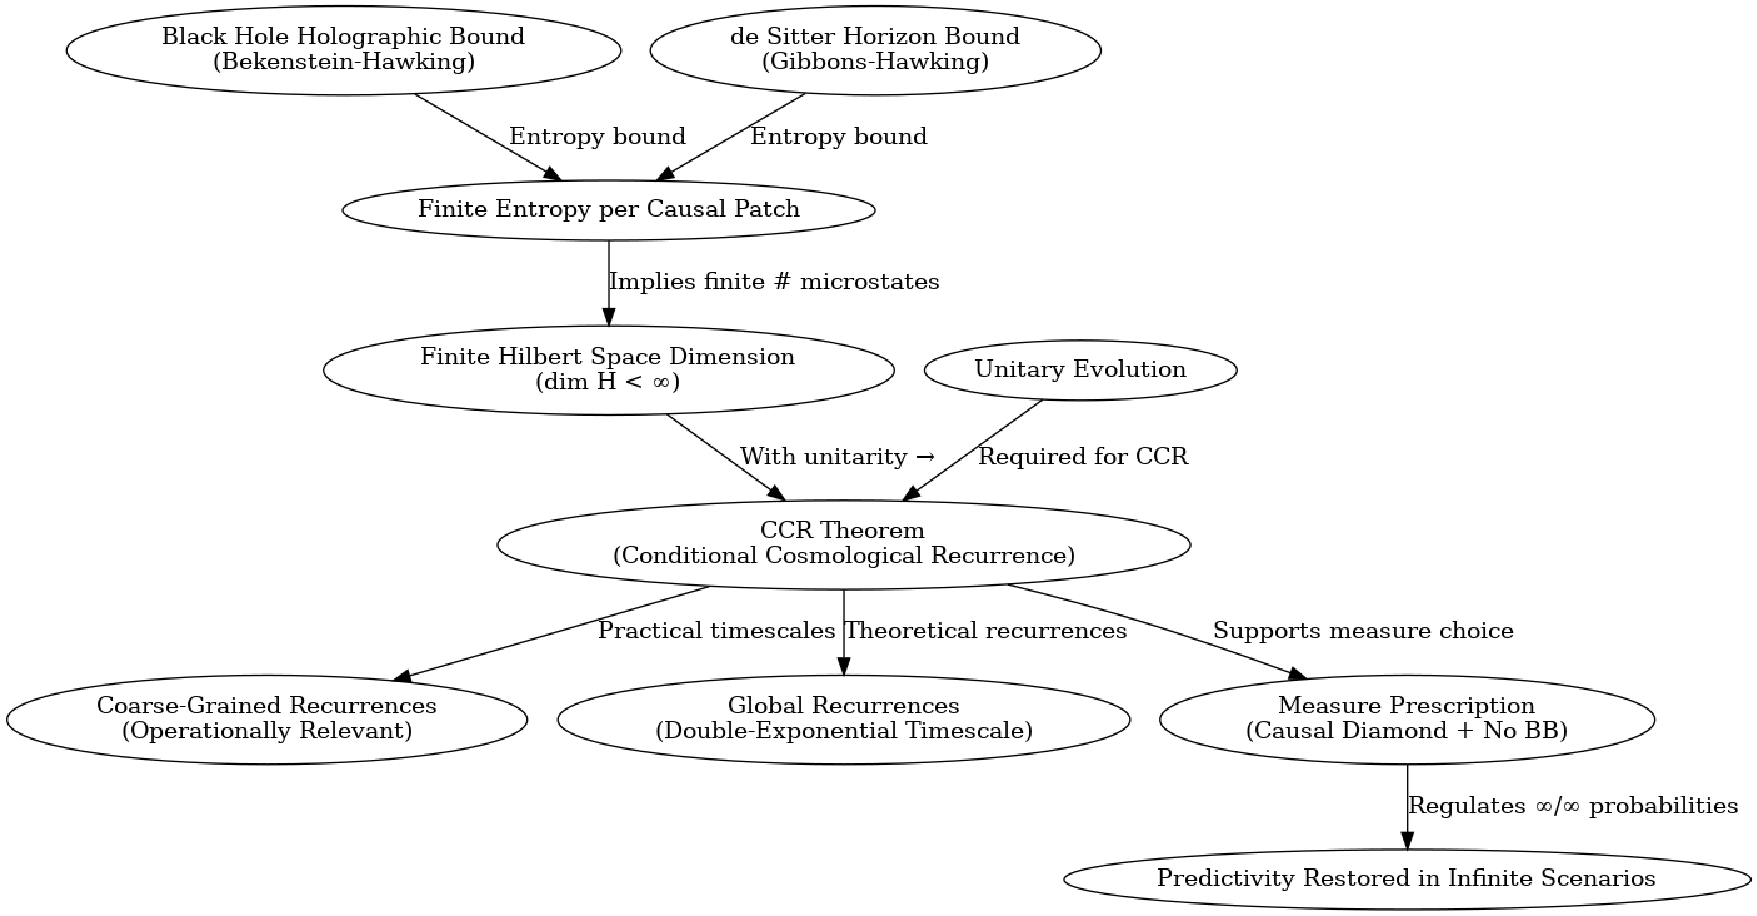
\includegraphics[width=0.9\linewidth]{ancillary_files/CCR_flowchart.pdf}
    \caption{Flow chart illustrating the logical structure of the CCR Theorem, from holographic bounds to conditional recurrences and their cosmological implications.}
    \label{fig:CCR_flowchart}
\end{figure}

\begin{table}[H]
\centering
\caption{Order-of-magnitude recurrence timescales for different scenarios. 
$S$ denotes the relevant entropy in units of $k_B$.}
\vspace{0.2cm}
\begin{tabular}{lccc}
\hline
\textbf{Scenario} & \textbf{$S/k_B$} & \textbf{$\Trec$} & \textbf{Observable?} \\
\hline
Global (de Sitter) & $10^{122}$ & $\exp\!\big(\exp(10^{122})\big)$ yrs & No \\
Coarse-grained subsystem & $10^{3}$ & $\exp(10^{3})$ yrs$^{\ast}$ & No \\
Toy model ($D=16$) & $\ln 16$ & $\sim 10^{2}$ units & Yes (verified) \\
\hline
\end{tabular}
\label{tab:timescales}
\end{table}
\vspace{-0.3cm}
{\footnotesize $^{\ast}$Still vastly exceeds the age of the universe.}

\section*{Appendix E: Methods for Toy Models}
\label{app:methods-toys}

\paragraph{Remark.}
The toy models presented in this appendix are intentionally minimal, serving
only as proofs-of-principle that finite Hilbert spaces generically imply recurrences.
They are not meant to quantitatively model cosmological dynamics. 
Future work could incorporate more sophisticated models (e.g.\ lattice field
theory truncations or AdS/CFT toy setups) to assess the robustness of these
scaling behaviors in settings closer to cosmology.


\paragraph{Global signal (finite-$D$).}
Random energy spectra $\{E_j\}_{j=1}^D$ (band-limited) are generated with weights $\{p_j\}$ drawn from a Dirichlet distribution, representing the squared amplitudes $|c_j|^2$ of the initial state.
The global fidelity is computed as
\[
F(t) = \left| \sum_{j=1}^D p_j \, e^{-i E_j t} \right|^2 .
\]
The global recurrence time $\Trec^{(\varepsilon)}$ is defined as the first $t>0$ such that $F(t) \geq 1-\varepsilon$, with $\varepsilon \in \{10^{-2}, 10^{-3}\}$.

\paragraph{Local proxy.}
For modeling coarse-grained or subsystem returns, a reduced set of $M$ modes $\{\omega_k\}$ with weights $\{q_k\}$ is employed, computing
\[
\mathcal{R}_A(t) = \left| \sum_{k=1}^M q_k \, e^{-i \omega_k t} \right| .
\]
The local recurrence time $\TrecA(\varepsilon_A)$ is the first $t>0$ where $\mathcal{R}_A(t) \leq \varepsilon_A$ (here $\varepsilon_A = 0.1$).
The scrambling time $\tscr$ is taken as the earliest $t$ when $\mathcal{R}_A(t)$ reaches $90\%$ of its late-time plateau value.

\paragraph{Numerics.}
All times are obtained from discrete time sampling with $\Delta t = 0.1$ up to $t_{\max} = 100$, 
using ensembles of $10^3$ realizations to estimate median values.

\clearpage
\section*{Appendix F: Scaling of Recurrence Times}

\emph{
\paragraph{Disclaimer.}
The following derivation is schematic: it provides order-of-magnitude scaling
estimates rather than exact recurrence times. The intent is to illustrate why,
under holographic entropy bounds, global recurrences are generically
double--exponential in $S/k_B$. Precise control requires number-theoretic
bounds on Diophantine approximation, which only reinforce (rather than weaken)
the double--exponential growth quoted here.
}

A standard estimate for recurrence times follows from the finiteness of the Hilbert space 
dimension $D$. For a generic Hamiltonian with $D$ nondegenerate energy levels, the 
quantum recurrence time scales as 
\begin{equation}
   T_{\mathrm{rec}} \sim \exp(D).
\end{equation}
Intuitively, this reflects the need to resolve phase differences among $D$ distinct 
frequencies. 

Meanwhile, holographic entropy bounds imply 
\begin{equation}
   D \sim \exp\!\left(\frac{S}{k_B}\right),
\end{equation}
where $S \lesssim S_{\max} \sim A/(4 \ell_P^2)$ is the Bekenstein--Hawking entropy 
associated with the causal patch. 

Combining these relations gives
\begin{equation}
   T_{\mathrm{rec}} \sim \exp\!\left[\,\exp\!\left(\tfrac{S}{k_B}\right)\right],
\end{equation}
i.e.\ a double-exponential scaling in the entropy. This simple derivation justifies the 
order-of-magnitude remark given in the main text (Remark~1).

A more refined treatment replaces the heuristic estimate $T_{\mathrm{rec}} \sim \exp(D)$ 
with bounds from Diophantine approximation on $D$-dimensional tori. 
Specifically, the recurrence time is controlled by the degree to which the energy 
gaps $\{E_j - E_k\}$ avoid low-order rational relations (Kronecker-type theorems). 
Metric results in simultaneous Diophantine approximation then imply that, 
for generic spectra, $T_{\mathrm{rec}}$ grows at least exponentially with $D$, 
leading again to the double-exponential scaling in $S/k_B$ quoted above.

\end{document}